\section{The \SYSTEM{} Approach} \label{sec:approach}

In this section we detail the \SYSTEM{} approach: a practical defense against
receiving corrupted or compromised resources over the internet. We further
present our proof-of-concept Google Chrome extension implementations, \DNSSYS{}
and \DHTSYS{}.

\subsection{Defeating User Apathy}

Human factors such as user apathy have stymied cryptographers for decades.
Schemes that are otherwise reasonably cryptographically solid can fail
catastrophically due to human error, confusion, or simple lack of interest. Some
users are likely to avoid using a security measure altogether if it presents
even a minor obstacle to immediate gratification~\cite{Clickthrough, PGPBad}. In
the browser, for example, this phenomenon can be observed empirically.

\begin{figure}[t]
    \centering
    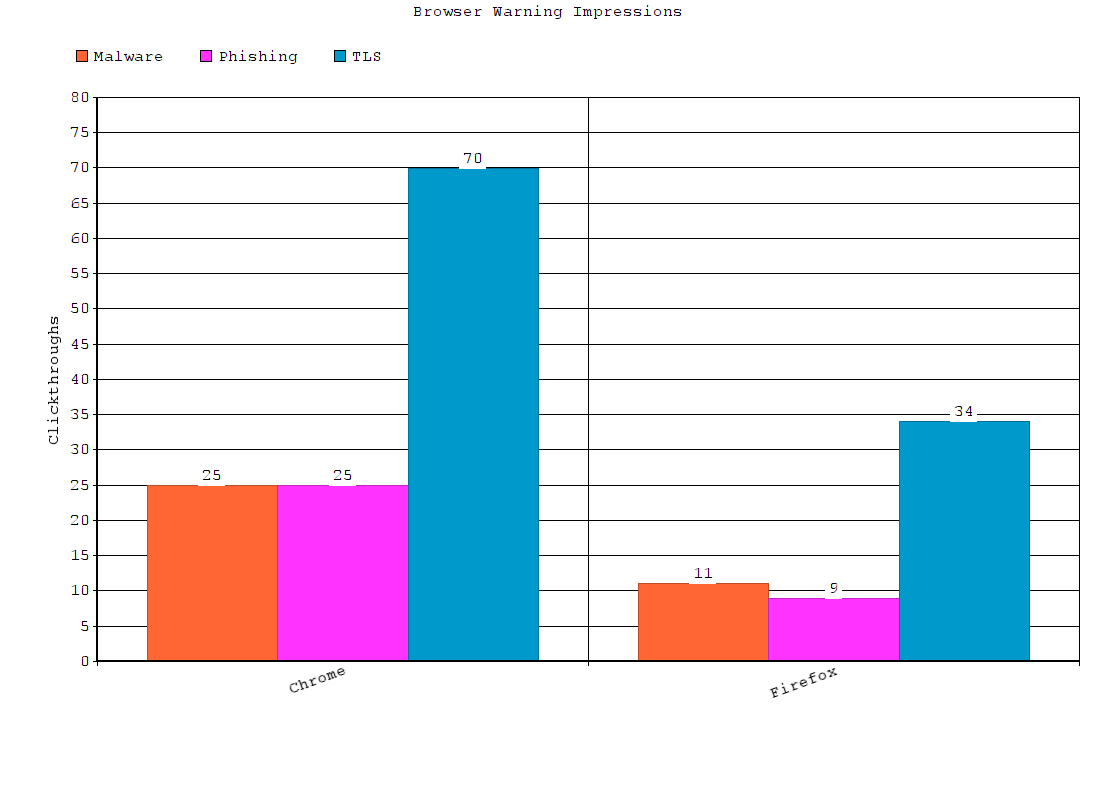
\includegraphics[width=0.95\linewidth]{impressions.png}
    \caption{Akhawe et al. estimation of warning clickthroughs by users as a
    percentage of total warnings observed for two popular
    browsers.}\label{fig:telemetry}
\end{figure}

Leveraging the in-browser telemetry of Mozilla Firefox and Google Chrome to
passively observe over 25 million warning impressions in 2013 (see
\figref{telemetry}), Akhawe et al. found that users of Google Chrome clicked
through a \emph{quarter of malware and phishing warnings} and \emph{70\% of TLS
warnings}~\cite{Clickthrough}. Users also clicked through a third of Mozilla
Firefox's TLS warnings and a tenth of their malware and phishing warnings. That
is to say: a significant percentage of browser users are \emph{determined} not
to let TLS trust issues and/or the threat of malware prevent them from receiving
their desired content. Hence, we must assume: some non-trivial number of users,
similarly determined to transact resources over the internet, will not be
burdened with the off-path minutiae of manually calculating a checksum (if they
are even familiar with the jargon) and verifying the integrity of the resources
they are downloading.

With this assumption in mind, the primary goal of \SYSTEM{} then is to side-step
the human factor altogether by providing a completely transparent and
unobtrusive in the average case, fully-automated method of checksum calculation
and verification in the average case that requires no changes to application
logic or source code. We achieve this through 1) the unique identification of
individual hosted resources and 2) a highly available mapping of unique resource
identifiers to corresponding checksums.

\PUNT{Next time :( \figref{overview} illustrates the \SYSTEM{} approach.}
\SYSTEM{} implementations can be imagined as a security layer sitting between
the user and the resource. Immediately after a resource is downloaded, two
cryptographic digests are generated. One digest uniquely fingerprints said
resource based on its name. This is known as the \emph{Non-Authoritative
Checksum} (NAC) and is yielded from running the cryptographic hashing function
over the contents of the resource file. The second digest uniquely fingerprints
said resource based on its contents. This is known as the \emph{Resource
Identifier} (RI) and is yielded from running the cryptographic hashing function
over the resource's public path on the distribution system.

Next, \SYSTEM{} uses the RI to retrieve an \emph{Authoritative Checksum} (AC)
from the backend. If successful, \SYSTEM{} will compare the NAC to the AC---we
refer to this as \emph{Non-Authoritative Checksum Validation} (NAC Validation).
In the case where NAC Validation fails, \ie they do not match, some
implementation-specific action should be taken to mitigate as much as possible
the risk to the end user. In most contexts, this means deleting or renaming the
unsafe resource, forcing the user to deal with the problem. Otherwise, \SYSTEM{}
remains completely transparent the the end user, as demonstrated by our
browser-based implementations.

\subsection{Defeating Co-Hosting}

Funding and maintaining a single server/system to host all of your assets can be
extremely cost-effective in the short term compared to hosting two or more
discrete systems---one hosting the resource and one hosting the resource's
checksum. Unfortunately, this establishes a single point of failure: an attacker
that compromises such a system can both mutate the resource and update the
checksum to match the mutation. Hence, \emph{co-hosting} a resource and its
corresponding checksum on the same distribution system virtually negates the
effectiveness of having a checksum at all. This is widely understood in the
security community~\cite{SCA-MINT2}.

Hence, deployment of \SYSTEM{} necessitates the existence of a separate
distribution mechanism for resources and for ACs. Though the concept of using
some distributed authenticated storage service to query a global mapping between
RIs and ACs is not new and seems straightforward, but the problem is more
complex than perhaps first meets the eye.

The state of the art in modern fully authenticated highly available schemes are
based on some form of PKI; an entity must roll its own PKI solution,
actively maintain it, and hope it is bug free. Examples include the Windows
Store, Google Play Store for Android, and the Apple Store for iPhone.

There are several problems with purely PKI-based resource integrity
verification. For one: a roll-your-own PKI-based model clearly cannot scale to
secure \emph{arbitrary} resources on the entire internet. This is doubly true
when considering the primary consumers of those resources---end users---likely
cannot distinguish a digital signature from, for instance, a key~\cite{PGPBad}.
Further, unlike a standardized approach like HTTPS/TLS or DNSSEC, which are
notoriously hard to implement correctly in their own right, rolling your own
PKI-based solution is a path fraught with even greater peril. It is well known
in the community that these often very complex PKI systems are hard to design
correctly, hard implement correctly, and hard to effectively maintain.

Fortunately, there has been a lot of effort put into researching, designing, and
standardizing several high availability fully authenticated globally distributed
high performance storage technologies, some of which web-facing entities and IT
teams are already quite familiar with and most already pay for, \eg the Domain
Name System (DNS). Adding extra resource records to a DNS zone, for instance, is
essentially a costless operation, meaning any entity that already has a
DNSSEC-protected web presence can immediately deploy \SYSTEM{}. This is key to
the motivation behind the \SYSTEM{} approach as well as the design of our
\DNSSYS{} proof-of-concept implementation.

Other candidate high availability systems include DHTs, storage clusters,
relational and non-relational databases, and any high availability authenticated
key-value store.

\subsection{Platform Diversity}

From our evaluation (cf. \secref{evaluation}), the computational overhead of
running \SYSTEM{} is minimal for most resources. Further, additional network
load is negligible. Hence, the \SYSTEM{} approach can be incorporated into
software on most any device capable of communicating with the chosen backend.
This includes desktops, laptops, tablets, mobile devices, embedded systems, etc.

\subsection{Proof-of-Concept Implementations}

\subsubsection{\DNSSYS{} and \DHTSYS{}}

We implement \SYSTEM{} as two proof-of-concept Google Chrome extensions:
\DNSSYS{} and \DHTSYS{}. They work with DNS and Ring OpenDHT as their highly
available backends, respectively. Our Chrome extensions do not make any
modifications to the Chrome user interface or viewport other than the extension
icon in the toolbar. Further, downloads work exactly the same whether or not
\DNSSYS{} or \DHTSYS{} are installed; the extensions are transparent to end
users. However, if a failure is experienced during NAC Validation (\ie a
``non-average'' case), the extensions will alert the user to the dangerous
download via toolbar icon and popup interface.

Immediately after a resource download is first detected, the extensions compute
an RI from the full URL path of the resource. For the purposes of our
proof-of-concept implementations, we calculate the RI as a hash digest of the
path component of the URL pointing to the resource. For example, consider a web
resource hosted at \texttt{https://somesite.com/var/downloadme.txt}. Our
implementations would hash \texttt{/var/downloadme.txt} to yield an RI. Note
that there are several ways a browser extension could calculate an RI. See
\secref{discussion} for a discussion of an alternative calculation based on
Uniform Resource Name.

Next, we determine the so-called \emph{Origin Domain} (OD). The OD is the base
domain used to query the backend and should always be the Second-Level Domain
(SLD) fragment of the \emph{active browser tab's URL}, \ie the URL of the tab
that initiated the download. For example: \texttt{somesite.com} would be the OD
for a Chrome tab at URL \texttt{frag.something.somesite.com} and
\texttt{fakesite.io} would be the OD for a Chrome tab at
\texttt{git.fakesite.io}.

The OD is appended to the Primary Label (PL), which is then appended to the
RI Sub-Label (SL). The PL is a standard string used to more easily identify the
backend records our implementations rely upon; we used ``\_dnschk''. It will
always appear as the third-level domain following the OD in any query to the
backend. The SL is a standard string used to identify backend entries that
contain RIs; we used ``\_ri'' in our implementations. The resulting
construction, consisting of \texttt{SL.PL.OD} (\eg
\texttt{\_ri.\_dnschk.fakesite.io}), is appended to the RI calculated earlier.
This forms the subject of the query to our backend, whereafter the backend
responds with the AC or an indication that the RI-to-AC mapping was not found.

To remain in compliance with DNS protocol label limits, we chose to split the
RI---a 64 character alphanumeric string---into two labels separated by a period.
We do this for both implementations, though it is only relevant with \DNSSYS{}.

The ultimate query sent to the backend consists of an OD (\eg
\texttt{fakesite.io}), a PL (static; \ie \texttt{\_dnschk}), an SL (static; \ie
\texttt{\_ri}), and an RI broken into two parts (\ie \texttt{RI1} and
\texttt{RI2}). This yields the following (with an example on line 2): \\
\makebox[\linewidth]{\texttt{RI1.RI2.SL.PL.OD}}
\makebox[\linewidth]{\texttt{RI1.RI2.\_ri.\_dnschk.fakesite.io}}

Finally, the backend responds to our query and NAC Validation is performed. If
NAC Validation succeeds, our extensions render a ``safe'' judgement via the
extension UI. If NAC Validation fails, our extensions render an ``unsafe''
judgement. If the backend response indicates the RI mapping we queried does not
exist, there are two possible outcomes: the extensions render a ``neutral''
judgement if they are not operating under strict mode conditions, otherwise an
``unsafe'' judgement is rendered (as if NAC Validation had taken place and
failed).

``Strict mode'' status, if active, prevents \DNSSYS{} and \DHTSYS{} from
rendering ``neutral'' judgements for a particular OD. The point of neutral
judgements is to allow the \SYSTEM{} approach to be incrementally adopted and
deployed on the open internet without ``breaking the internet'' or pestering the
end user with false positives when downloading resources that are not explicitly
protected by our approach. For resources that are protected by our approach,
strict mode ensures there are only two possible judgements rendered by \DNSSYS{}
and \DHTSYS{} for a given OD: either ``safe'' if NAC Validation succeeds or
``unsafe'' in all other circumstances. For this reason, it is recommended that
any adopter of our approach ensure their resources are protected under strict
mode by default.

To determine if strict mode status applies to an OD, an additional backend query
is made of the form \texttt{SML.PL.OD}, where SML is the Strict Mode Sub-Label
consisting of the standard string ``\_smode''. Continuing with our previous
example, our query would take the form \texttt{\_smode.\_dnschk.fakesite.io}. If
and only if the subject of this additional query exists in the backend, strict
mode status is assumed.

\subsubsection{Determining Origin Domain in the Browser}

To execute a resource integrity attack on a web server, an attacker generally
has two paths. They can mutate the resource in place, which would cause NAC
Validation to fail. They could also mutate the web page hosting the resource,
replacing the resource anchor with a malicious one that points to a compromised
resource on the attacker's remote system. \DNSSYS{} and \DHTSYS{} will catch
this due to how we calculate the Origin Domain (OD).

To prevent such implementation-specific attacks, we make a distinction between
the domain a resource's hyperlink might be pointing to (which might belong to
the attacker) and the OD, which is the domain of the web document that contains
said hyperlink. The scope of the OD is at the tab level, meaning there is one OD
determined for each open browser tab.

In our proof-of-concept implementations, we rely on the Chrome Tabs and
WebRequest APIs to associate downloads with ODs. Our extensions are implemented
such that the OD is determined as early as possible in a Chrome tab's navigation
lifecycle. Further, in our implementations, determined ODs are ultimately
ordered as a LIFO construction. This ensures the resource-to-tab mappings remain
accurate in the case where two tabs share the same OD when a resource download
is observed.
